\section{Holdings, trading and mechanism evidence}
\subsection{Benchmark linked holdings and the denominator problem}

Table~\ref{tab:demand} relates returns to reported holdings changes on a common sample. For additions, mean C-group purchases rise from 0.15\% of shares outstanding in 2007--2011 to 1.11\% in 2017--2021, before declining to 0.97\% in 2022--2026. These are changes in observed fund ownership, not estimates of the total amount of passive capital tracking the index. The first comparison is particularly fragile because it involves only eight addition events across five reviews. Figure~\ref{fig:demand} displays the annual series without implying that its changing coverage is economically neutral.

\begin{table}[!htbp]
\centering
\caption{Returns scaled by observed benchmark linked fund purchases}\label{tab:demand}
\small
\setlength{\tabcolsep}{5pt}
\begin{tabular}{llrrrrrl}
\toprule
Type & Period & $N$ & $G$ & $\bar Y$ & $\bar D_C$ & $\widehat M$ & Fieller set \\
\midrule
Addition & 2007--11 & 8 & 5 & 8.78 & 0.15 & 57.87 & [-9.55, 471.88] \\
Addition & 2012--16 & 27 & 8 & -1.94 & 0.52 & -3.76 & [-15.09, 4.24] \\
Addition & 2017--21 & 58 & 10 & 3.29 & 1.11 & 2.97 & [-0.14, 6.30] \\
Addition & 2022--26 & 78 & 9 & 2.28 & 0.97 & 2.35 & [-0.21, 4.73] \\
Addition & 2017--26 & 136 & 19 & 2.71 & 1.03 & 2.63 & [0.91, 4.37] \\
Deletion & 2007--11 & 7 & 3 & -0.19 & 0.26 & -0.72 & All real values \\
Deletion & 2012--16 & 25 & 7 & 2.07 & 0.48 & 4.36 & [-17.73, 30.17] \\
Deletion & 2017--21 & 40 & 10 & 0.20 & 0.99 & 0.20 & [-4.05, 4.89] \\
Deletion & 2022--26 & 68 & 9 & 1.66 & 1.18 & 1.41 & [-0.87, 2.83] \\
Deletion & 2017--26 & 108 & 19 & 1.12 & 1.11 & 1.01 & [-0.88, 2.61] \\
\bottomrule
\end{tabular}
\begin{minipage}{\linewidth}\footnotesize\vspace{5pt}
$Y=s_i CAR_i[AD-1,ED+1]$ and $D_C$ is the sign-adjusted change in covered benchmark-linked funds\textquotesingle{} holdings as a percentage of shares outstanding; $s_i=1$ for additions and $-1$ for deletions. Positive values therefore indicate movement in the index-directed direction for both event types. $\widehat M=\bar Y/\bar D_C$ uses the same non-split complete-case sample for both means. Group C includes strict followers, benchmark variants, and benchmark-linked mixed-fund holdings. The last column is a 95\% Fieller confidence set using the joint CR1 covariance of both means and $t_{G-1}$, an asymptotic sensitivity measure rather than exact small-sample inference. It differs from the inherited percentile bootstrap. Source: fund\_demand/omrakning\_resultat.csv, table 5, and audit/results/fieller\_ratios.csv.
\end{minipage}
\end{table}


The early addition ratio is 57.87 percentage points of CAR per percentage point of covered ownership change. It would be tempting to compare this with 2.35 in the latest block and describe an extraordinary increase in the elasticity of stock supply. That conclusion is not warranted. The early denominator is small, the numerator is imprecise, and the observed investor set expands over time. The 95\% Fieller set for the early ratio runs from -9.55 to 471.88. Even its sign is not precisely resolved by this calculation. The earliest deletion sample is weaker still: seven observations across three reviews produce a Fieller set containing every real value.

For later additions, the holdings measurement is better supported. Pooling 2017--2026 yields a common-sample return of 2.71\%, a C-group ownership change of 1.03\%, and a ratio of 2.63. Its Fieller interval is [0.91, 4.37]. This supports a positive association between the measured numerator and a positive measured demand denominator in the later pooled sample. It does not validate the ratio as a structural inverse elasticity. Some of the measured trading may respond to the same information that moves prices, and the reporting interval is broader than the return window.

The period-specific inference is less decisive. The 2017--2021 and 2022--2026 addition Fieller sets both include zero, even though their inherited percentile-bootstrap intervals do not. The distinction arises because the procedures summarize joint numerator-denominator uncertainty differently. Neither is an automatic gold standard with nine or ten clusters. Reporting the discrepancy is more informative than selecting the narrower interval. For deletions, the later-decade ratio is 1.01 and its Fieller interval includes zero. Sign adjustment changes the direction convention; it does not make addition and deletion mechanisms symmetric.

\begin{figure}[!htbp]\centering
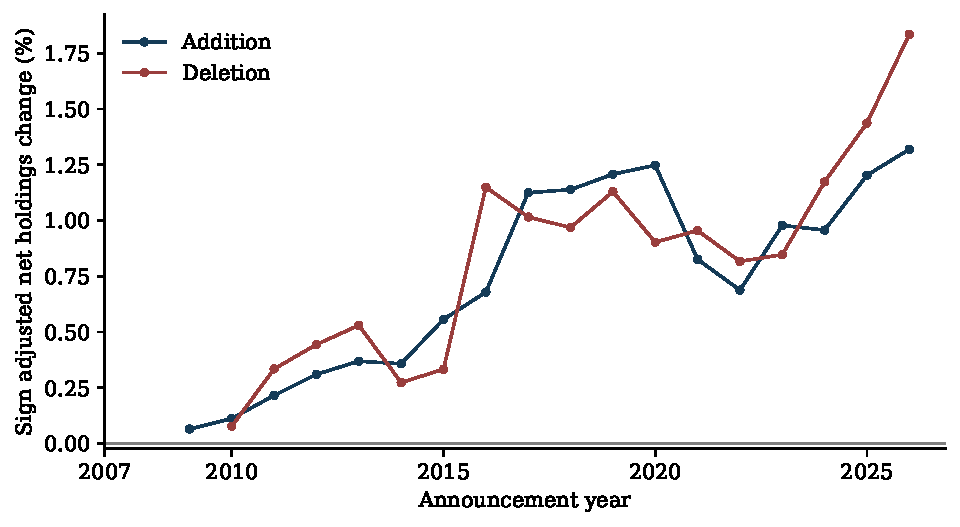
\includegraphics[width=.94\linewidth]{figures/fund_demand.pdf}
\caption{Measured ownership changes around index events. Annual means of sign-adjusted changes in C-group holdings as a percentage of shares outstanding. Positive deletion values indicate net sales. The series uses the holdings sample; coverage changes over time and 2026 is incomplete. It is neither total index-tracking assets nor implementation-day trading. Source: fund\_demand/figur1\_skikt.csv.}\label{fig:demand}
\end{figure}

An independent reporting channel provides a useful measurement comparison. In the matched 2019--2026 addition sample with 106 events across 15 reviews, the Finansinspektionen-based ownership measure is 1.14\%, compared with 1.05\% for the matched C measure. The common-sample CAR is 2.43\%, giving ratios of 2.12 and 2.30, respectively. Their inherited bootstrap intervals are [0.87, 3.79] and [0.93, 4.15]. Agreement on this overlap is reassuring about scale for the observed later sample. It cannot establish full fund coverage, recover the missing early ownership denominator, or make holdings changes exogenous.

The economic conclusion from the holdings evidence is consequently limited but substantive. Benchmark-linked investors demonstrably change their reported positions around these events, and their observed trades are large enough that ignoring demand would be uninformative. The evidence does not tell us what fraction of the return is generated by those trades. Historical comparisons of price-to-demand ratios require comparable investor coverage, correctly adjusted share counts, and a credible separation of unexpected index demand from other trading. Those conditions remain research requirements rather than established facts.

\subsection{Trading concentrates before implementation}

Daily volume provides a different view of implementation. For each event, the inherited measure divides daily trading volume by total volume over ED-22 through ED+22, a 45-trading-day window. The final trading day before effectiveness accounts for 9.44\% of that volume for early additions and 15.24\% for latest-period additions. The change is 5.79 percentage points, with an inherited review-bootstrap interval of [3.30, 8.84]. Deletions show a similar rise, from 8.75\% to 14.52\%, a difference of 5.76 percentage points with an interval of [3.26, 8.38]. Figure~\ref{fig:volume} displays the surrounding daily profile.

\begin{figure}[!htbp]\centering
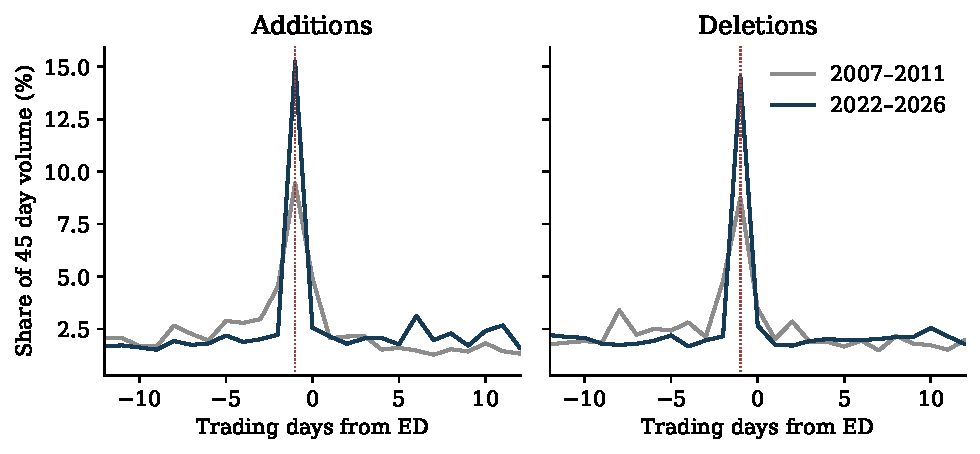
\includegraphics[width=.96\linewidth]{figures/volume_concentration.pdf}
\caption{Concentration of trading around effectiveness. Average daily shares of each event's total volume over ED-22 to ED+22. The figure shows ED-12 to ED+12 from that fixed denominator. The dotted line marks ED-1. Missing volume is set to zero in the inherited calculation; volume-sample counts therefore differ from complete return counts. Daily observations do not distinguish auctions from continuous trading. Source: liquidity/volume\_share\_by\_day.csv.}\label{fig:volume}
\end{figure}

This concentration and the recent small implementation-window return are not contradictory. A larger share of activity can occur on a particular day while the equilibrium price adjustment remains small. Investors may trade against anticipated demand; the supply of immediacy may have improved; or prices may already incorporate information about likely membership. The data do not separately identify those explanations. In particular, a volume share is not total turnover, and it cannot measure the execution costs paid by a benchmark fund. A smaller denominator elsewhere in the window could also increase the share.

The analysis is descriptive in two further respects. Events are averaged without equalizing their investment capacity or economic importance. The treatment of missing volume as zero can affect concentration if missingness changes over time. Reconstructing complete intraday trading and auction data would be necessary to distinguish a true shift toward closing-auction execution from changes in daily reporting and trading outside the event day.

\subsection{Quoted spreads and observable liquidity}

The broader market panel shows a decline in the value-weighted closing quoted spread of OMXSB members, from 0.270\% in 2007 to 0.079\% in 2025. The partial 2026 observation is 0.087\%. The measure is the closing ask-minus-bid spread relative to the quote midpoint; quotes above 20\% are removed in the inherited construction. Figure~\ref{fig:spread} describes the evolution without attributing it to index trading.

\begin{figure}[!htbp]\centering
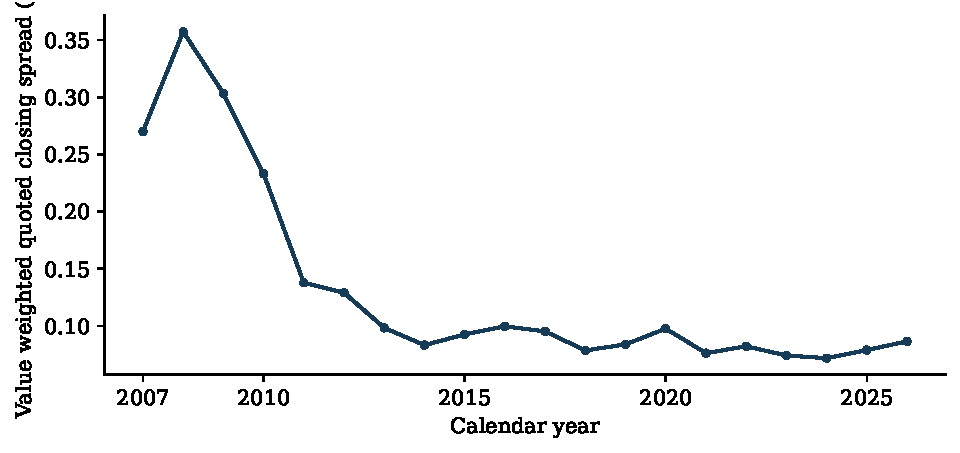
\includegraphics[width=.94\linewidth]{figures/quoted_spread.pdf}
\caption{Quoted closing spreads among index members. Calendar-year averages of the value-weighted quoted bid-ask spread relative to the quote midpoint, in percent. The 2026 observation is incomplete. This is an observable quote measure, not an effective spread, implementation shortfall or causal measure of liquidity provision. Source: liquidity/spread\_by\_year.csv.}\label{fig:spread}
\end{figure}

Lower quoted spreads are consistent with a market in which smaller trades can be executed more cheaply. They do not directly measure the slope of residual stock supply for a large index-related order. That slope depends on market depth, inventory capacity and the response of other investors, none of which is fully captured by the closing spread. The weighting also uses the available capitalization measure; multiple listed share classes and changing membership can affect the aggregate. The figure therefore gives institutional context for the return results, rather than a test that liquidity improvements caused their attenuation.

Taken together, holdings and volume indicate that small implementation-window returns do not mean index-related activity has become unimportant. The main uncertainty is about how much of the observed return reflects that activity, when any adjustment occurs, and how the relevant demand is measured. These distinctions motivate the robustness and horizon analyses rather than a single mechanism conclusion.
\FloatBarrier
